\chapter{Estudo de caso}
\label{cap:estudodecaso}

Neste trabalho será apresentada a estrutura de uma empresa que fornece serviços de hospedagens e também está associada a um provedor de 
internet\footnote{É importante salientar que esse provedor utiliza a maior parte dos serviços da empresa, pois possui maior número de clientes.}. 
A empresa possui grande parte de seus clientes localizados na serra do Rio Grande do Sul, sendo que atualmente essa empresa possui 
aproximadamente 9000 clientes. A sede da empresa está localizada na cidade de Garibaldi, além disso possui quatro filiais no estado, 
atendendo aproximadamente xx?? cidades. Essa empresa possui aproximadamente xx?? funcionários.

A empresa oferece serviços pela internet aos seus clientes, que são: hospedagens de sites, banco de dados, \textit{e-mail}, sistemas de gestão, 
\textit{e-mail marketing}, \textit{backup}, \textit{máquinas virtuais}, autenticação \ac{ADSL}, rádio \textit{online} e telefonia.
Além disso, o provedor associado fornece aos seus clientes acesso à internet via rádio e acesso à internet por meio de fibra óptica.
A maioria dos serviços são fornecidos por meio de \textit{softwares} de código aberto, que executam sobre sistemas operacionais, normalmente 
distribuições \textit{Linux}, e também são \textit{softwares} livre.

Atualmente a empresa possui redundância de refrigeração e de energia (Figura \ref{fig:insteletrica}). A redundância de refrigeração é composta 
por dois ares-condicionados. 
A redundância de energia é feita através de três \textit{nobreaks}, sendo que dois deles são utilizados para alimentação dos servidores e outros 
equipamentos como por exemplo roteadores, de uma forma que caso um falhar o outro alimente todos os equipamentos. O terceiro \textit{nobreak} é 
utilizado para alimentar os computadores dos funcionários de dois setores. Além disso, dois geradores suprem a necessidade de consumo de 
energia elétrica do ambiente.

\begin{figure}[h!]
 \centering
 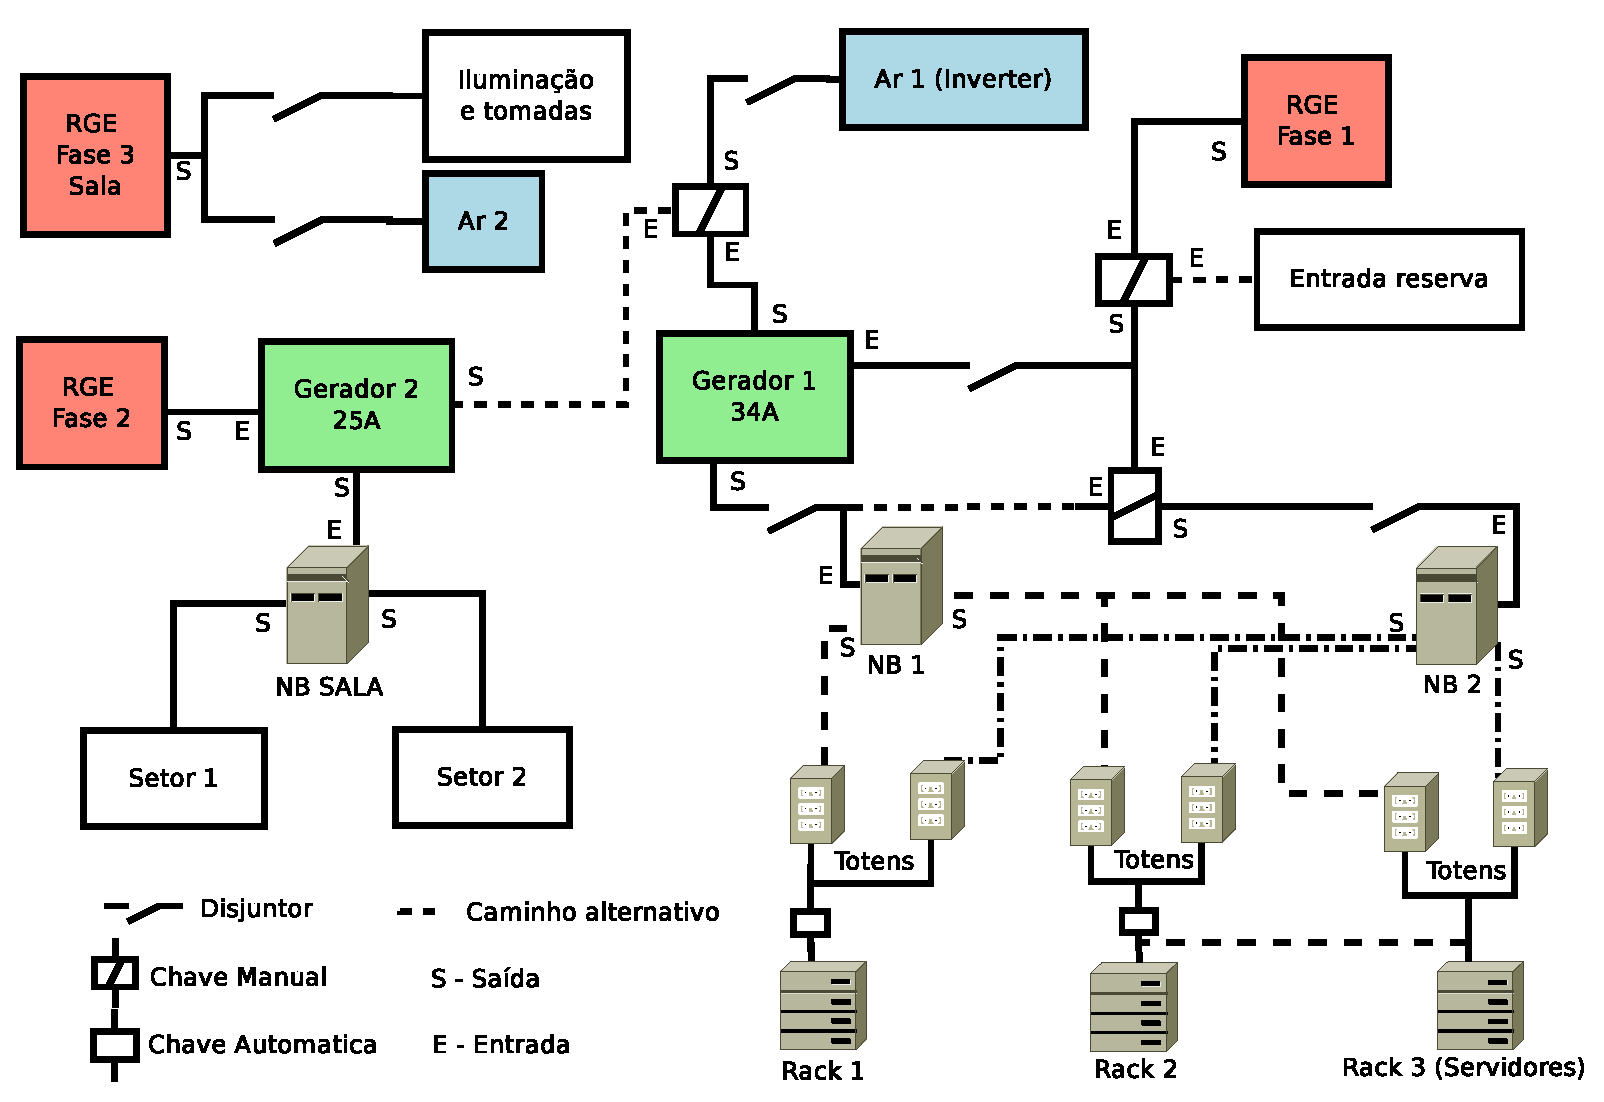
\includegraphics[width=380px]{img/insteletrica.eps}
 \caption{Diagrama de instalação elétrica.}
 \label{fig:insteletrica}
\end{figure}

Nas próximas seções serão detalhados: o ambiente físico dos servidores, com suas estruturas e suas configurações, além da estrutura de 
virtualização e todos os serviços fornecidos pelos servidores (Seção \ref{section:ambiente}), e por fim, a seleção dos serviços 
críticos (Seção \ref{section:servcrit}).

\section{Ambiente físico e virtual}
\label{section:ambiente}

A estrutura atual da empresa é composta por quatorze servidores físicos montados em um \textit{rack} (Figura \ref{fig:servrack}). 
A configuração de \textit{hardware} desses servidores encontradas na Tabela \ref{tab:servfisicos}, onde tem-se o nome do servidor, o modelo do 
servidor, a configuração dos processadores, quantidade de memória, número de discos e a capacidade unitária de cada disco.

\begin{figure}[h!]
 \centering
 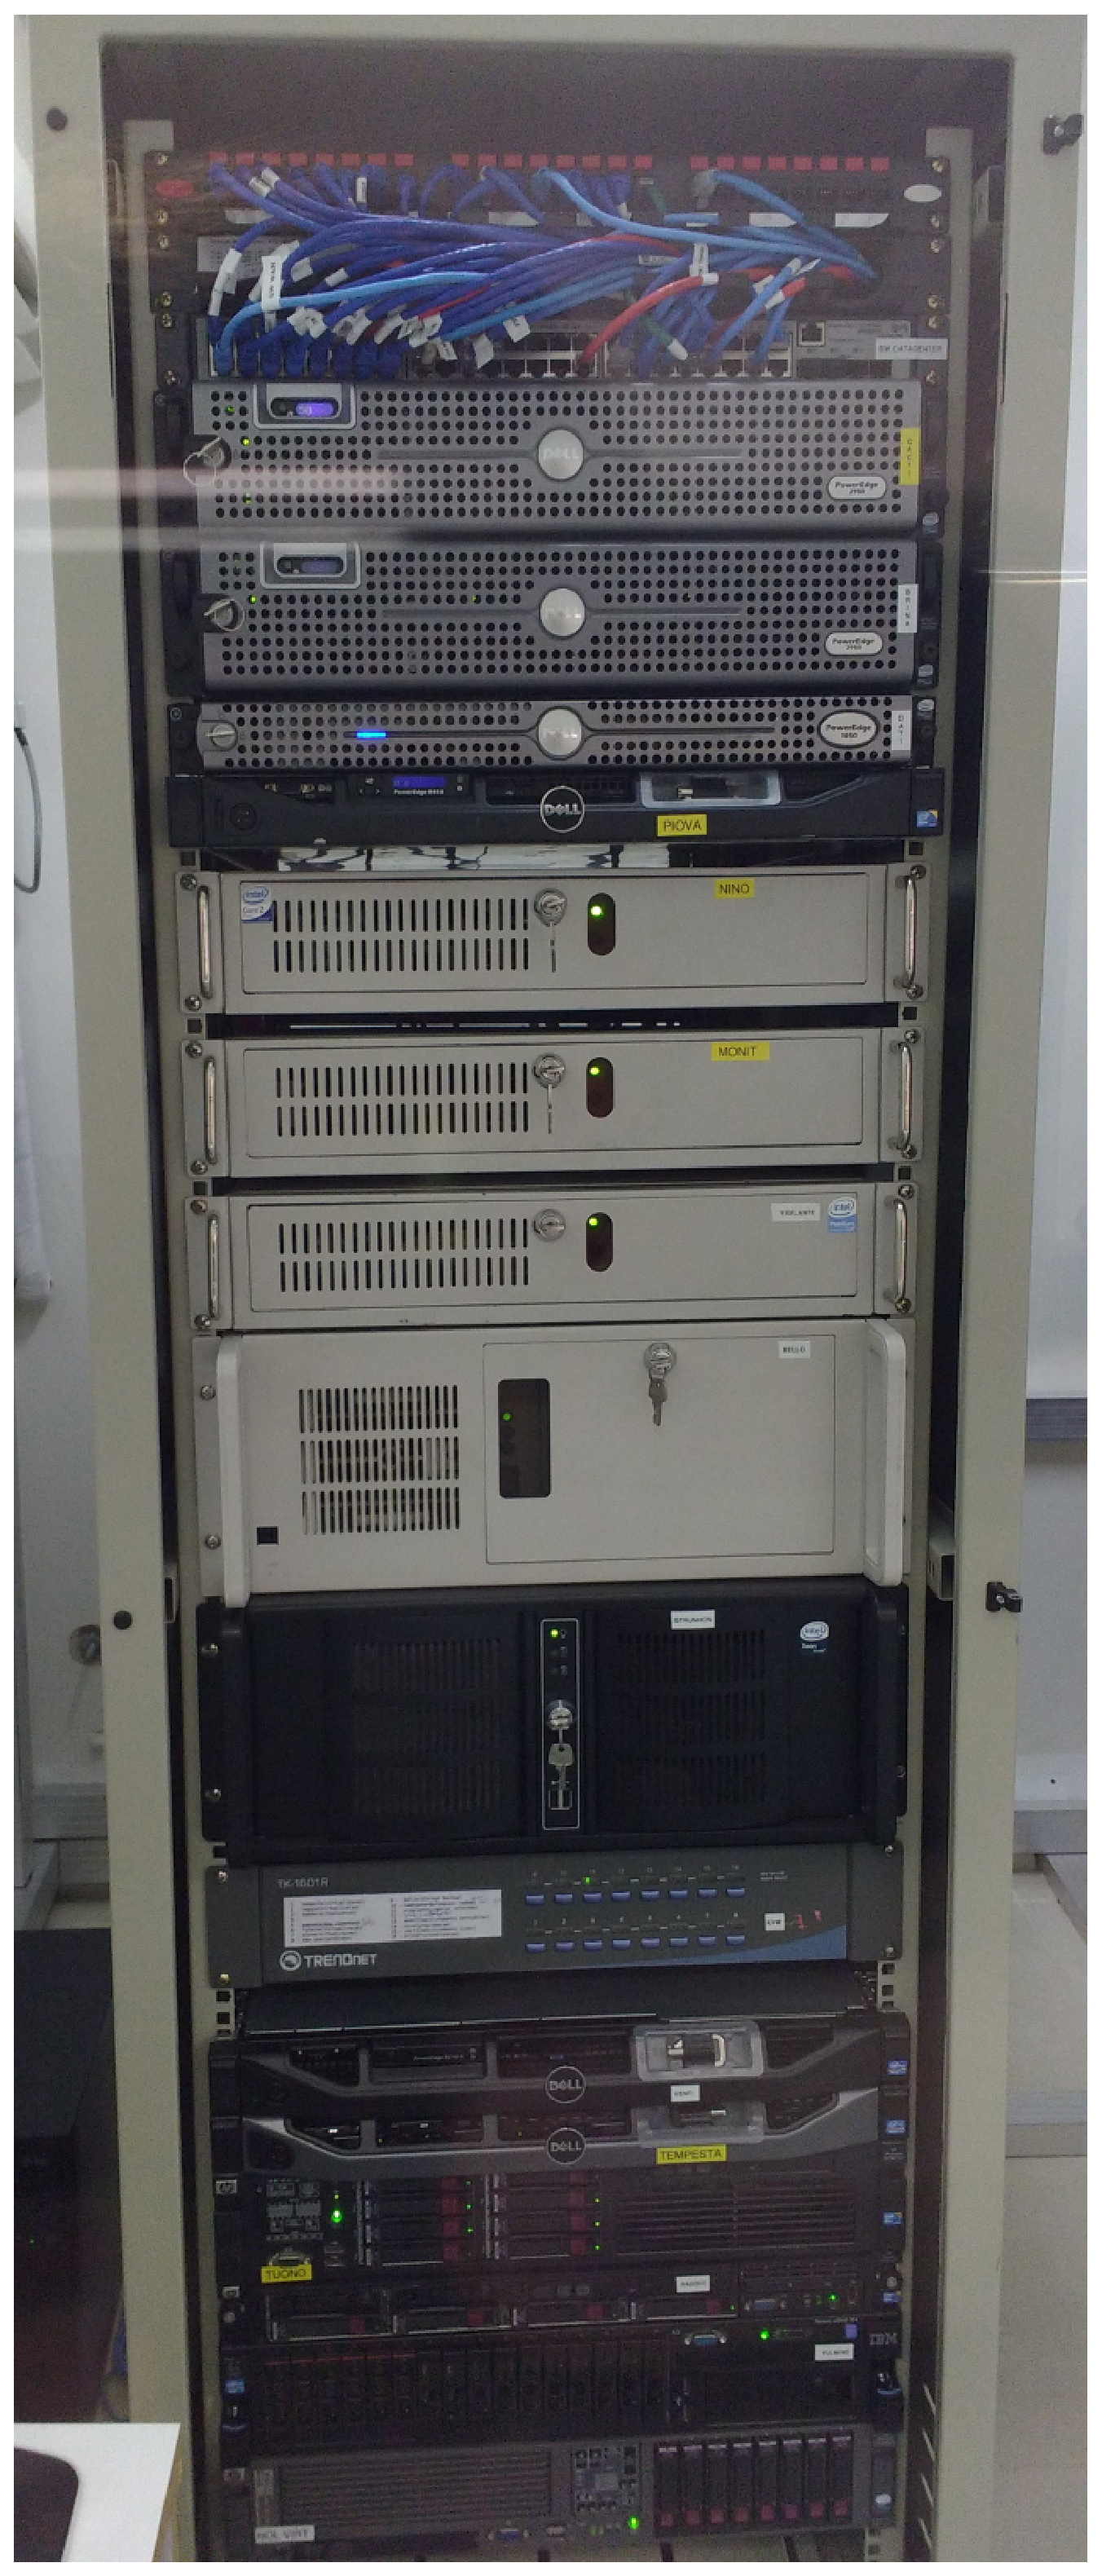
\includegraphics[width=200px]{img/servrack.eps}
 \caption{Imagem do \textit{rack} e dos servidores.}
 \label{fig:servrack}
\end{figure}

\begin{table}
\caption{Configuração dos servidores físicos.}
\label{tab:servfisicos}
\begin{center}
\begin{tabular}{|l|l|p{4cm}|l|p{2.1cm}|}\hline
Servidor & Modelo & Processador & Memória & Disco\\\hline
Bello & & 1 x Intel Core 2 Duo CPU E6750 2.66 GHz & 2 GB DDR2 & 5,5 TB SATA\\\hline
Cacti & Dell PowerEdge 2950 & 2 x Intel Xeon CPU E5310 1.60 GHz & 12 GB DDR2 & 2 x 73 GB SAS\\\hline
Dati & Dell PowerEdge 1850 & 2 x Intel Xeon CPU 3.20 GHz & 4 GB DDR2 & 2 x 146 GB SCSI\\\hline
Monit & & 1 x Intel Core 2 Quad CPU Q9550 2.83 GHz & 4 GB DDR2 & 120 GB SSD\\\hline
Nino & & 1 x Intel Core 2 Duo CPU E4500 2.20 GHz & 4 GB DDR2 & 500 GB SATA\\\hline
Sfrunhon & & 1 x Intel Xeon CPU X3330 2.66 GHz & 8 GB DDR2 & 750 GB SATA\\\hline
Vigilante & & 1 x Intel Pentium Dual CPU E2180 2.00 GHz & 4 GB DDR2 & 2,5 TB SATA\\\hline
Brina & Dell PowerEdge 2950 & 2 x Intel Xeon CPU E5410 2.33 GHz & 24 GB DDR2 & 6 x 300 GB SAS\\\hline
Fulmine & IBM System x3650 M4 & 1 x Intel Xeon CPU E5-2650 2.00 GHz & 32 GB DDR3 & 6 x 2 TB SATA\\\hline
Piova & Dell PowerEdge R410 & 2 x Intel Xeon CPU E5530 2.40 GHz & 32 GB DDR3 & 4 x 500G SATA\\\hline
Raggio & HP ProLiant DL360 G7 & 2 x  Intel Xeon CPU E5630 2.53 GHz & 32 GB DDR3 & 4 x 300 GB SAS\\\hline
Tempesta & Dell PowerEdge R620 & 2 x Intel Xeon CPU E5-2620 2.00 GHz & 32 GB DDR3 & 5 x 1 TB SATA 3 x 1,2 TB SAS\\\hline
Tuono & HP ProLiant DL380 G7 & 2 x Intel Xeon CPU E5649 2.53 GHz & 32 GB DDR3 & 6 x 300 GB SAS 2 x 146 GB SAS\\\hline
Venti & Dell PowerEdge R210 II & 1 x Intel Xeon CPU E3-1220 3.10 GHz & 16 GB DDR3 & 2 x 3 TB SATA\\\hline
\end{tabular}
\end{center}
\end{table}

Todos os servidores estão ligados ao \textit{switch}, que provê aos servidores acesso à internet através do roteador. 
Para os servidores mais importantes utiliza-se dois cabos de rede que estão ligados a um \textit{switch} \textit{gigabit}, assim possibilitando
a configuração de \textit{link aggregation}, que possibilita configurar mais de uma interface de rede física em uma interface agregada, com isso 
permitindo dobrar a capacidade de tráfego de dados e assim é caracterizado a redundância do cabeamento.
O diagrama da Figura \ref{fig:servfisicos} demonstra uma visão geral da estrutura física dos servidores da empresa, com dois exemplos de cada 
tipo de servidor. 

\begin{figure}[h!]
 \centering
 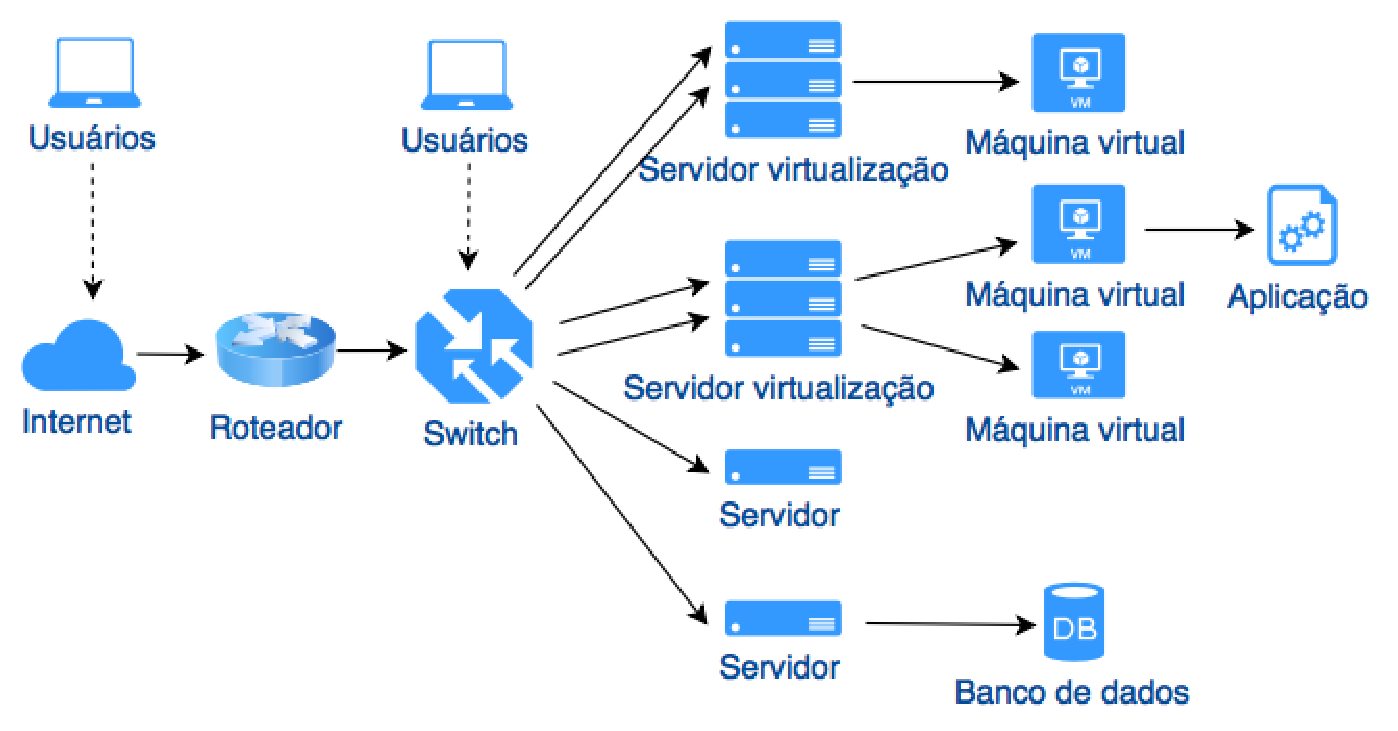
\includegraphics[width=430px]{img/servfisicos.eps}
 \caption{Estrutura física.}
 \label{fig:servfisicos}
\end{figure}

Existem sete servidores que possuem serviços executando sobre o sistema operacional nativo, ou seja, sem virtualização. Eles são os sete 
primeiros servidores da Tabela \ref{tab:servfisicos}:
\begin{itemize}
 \item Bello: esse servidor possui o sistema operacional \textit{Ubuntu 14.04 \ac{LTS}}. Sua função é armazenar dados de \textit{backup}, ele 
 possui \textit{storage} da ferramenta \textit{bacula} (pacote \textit{bacula-storage} versão ??) para \textit{backup} dos outros servidores;
 
 \item Cacti: um dos servidores de monitoramento da rede do provedor. Esse utiliza a distribuição \textit{CentOS 6.??} e executa a aplicação
 \textit{Cacti} versão 0.??, que é uma ferramenta de código aberto desenvolvida para monitorar equipamentos de rede. Ela monitora atualmente a 
 maior parte da rede \textit{core} e a rede \textit{backbone} tanto dos clientes de internet via rádio, como de fibra óptica;
 
 \item Dati: é o servidor de banco de dados principal. Esse possui o sistema operacional \textit{Ubuntu 14.04 \ac{LTS}}. O serviço que executa
 sobre esse servidor é um banco de dados \textit{MySQL} versão 5.5 ??, onde armazena os dados das aplicações de \textit{ZoneMinder} (servidor 
 de câmeras) e \textit{Icewarp Mail Server ??} (servidor de e-mail), que serão detalhados posteriormente;
 
 \item Monit: esse servidor faz o monitoramento de todos os servidores. Ele possui o sistema operacional \textit{Ubuntu 12.04 \ac{LTS}}.
 Suas aplicações são \textit{Nagios} versão 3.?? e \textit{Munin} versão 1.??, ambos \textit{softwares} livres. O primeiro monitora desde os 
 serviços de cada servidor, até o seu \textit{hardware}, para isso utiliza um cliente (\ac{NRPE}), que deve ser instalado em cada servidor, para 
 monitorar dados não acessíveis externamente, como espaço em disco, número de processos, falhas de \textit{hardware}, entre outros. O segundo, 
 \textit{Munin}, é responsável por gerar gráficos para ajudar com monitoramento, com ele pode-se criar por exemplo gráfico de processador, 
 memória, utilização de disco, e até temperatura e velocidade dos \textit{fans ??ac??} para alguns servidores;
 
 \item Nino: esse é o servidor utilizado pelo setor de desenvolvimento de \textit{software}. Suas aplicações executam sobre o sistema operacional
 \textit{Ubuntu 14.04 \ac{LTS}}. Os serviços fornecidos pelo servidor são: servidor \textit{web} (\textit{apache 2.4 ??} e 
 \textit{\ac{PHP} 5.6 ??}), banco de dados (\textit{MySQL 5.??} e \textit{PostgreSQL} 9.??), arquivos compartilhados?? (\textit{samba ??}), 
 controle de versões de \textit{software} (\textit{\ac{SVN} ??}), .. ?? ;
 
 \item Sfrunhon: outro servidor de monitoramento da rede do provedor. Esse utiliza a distribuição \textit{CentOS 6.??} e executa a aplicação
 \textit{Cacti} versão 0.??. Esse servidor monitora atualmente o trafego dos clientes, tanto de internet via rádio, como de fibra óptica;
 
 \item Vigilante: esse servidor é responsável por capturar e armazenar \textit{streaming} de vídeo de câmeras do provedor. Esse servidor possui
 o sistema operacional \textit{Ubuntu 14.04 \ac{LTS}}. O servidor executa a aplicação \textit{ZoneMinder}, que também é uma ferramenta de códito 
 aberto, para capturar e armazenar as imagens das câmeras do provedor.
\end{itemize}

%\section{Serviços e virtualização ?}
%\label{section:servicos}

Os servidores de virtualização possuem suas respectivas \ac{VM}s, que executam aplicações. Para virtualização utiliza-se o hipervisor 
\ac{KVM} e a ferramenta \textit{QEmu}, sendo que ambos são projetos de \textit{software} livre. Procurou-se manter um ambiente homogêneo?? 
com o objetivo de facilitar a manutenção, para isso utilizou-se o mesmo hipervisor e o mesmo sistema operacional, esse sistema operacional é
o sistema de código aberto \textit{Ubuntu 14.04 \ac{LTS}}.
Além disso, esses servidores possuem redundância de \textit{hardware}, com fonte de alimentação e discos configurados através de um \ac{RAID}, 
geralmente utilizando \ac{RAID} 5, em alguns casos, que possui apenas dois discos é utilizado \ac{RAID} 1. O ambiente também possui uma 
redundância do cabeamento, como visto anteriormente.

A empresa fornece serviços diversos, desde hospedagens de sites até \ac{DNS} recursivo para o provedor de internet. Atualmente sete servidores 
são utilizados para virtualizar sistemas, esses servidores são os últimos sete servidores da Tabela \ref{tab:servfisicos}.
Sendo que existem quarenta e seis \ac{VM}s distribuídas entre os sete servidores de virtualização.
Para melhor entender, a seguir será descrito esses servidores e suas respectivas máquinas virtuais.

O servidor Brina possui ?? \ac{VM}s, que executam os serviços (Figura \ref{fig:servlog1}):
\begin{itemize}
 \item \textit{Merak}: esse servidor virtual fornece serviço de e-mail. Ele possui uma configuração de quatro \textit{cores} para processamento, 
 8 GB de memória e 1000 GB de disco. O servidor possui o sistema operacional \textit{Windows 2008 Server R2 ??} e executa o \textit{software} 
 \textit{Icewarp Mail Server ??}. Essa aplicação fornece os serviços de envios de e-mails (\ac{SMTP}), recebimentos de e-mails (\ac{POP} e 
 \ac{IMAP}), Webmail (\ac{PHP}), ?? ... Possui ?? contas sendo que possui uma média de ?? usuários simultâneos...
 Grande parte das contas estão ociosas pois são oferecidas juntamente com a internet vendida pelo provedor.

\end{itemize}

\begin{figure}[h!]
 \centering
 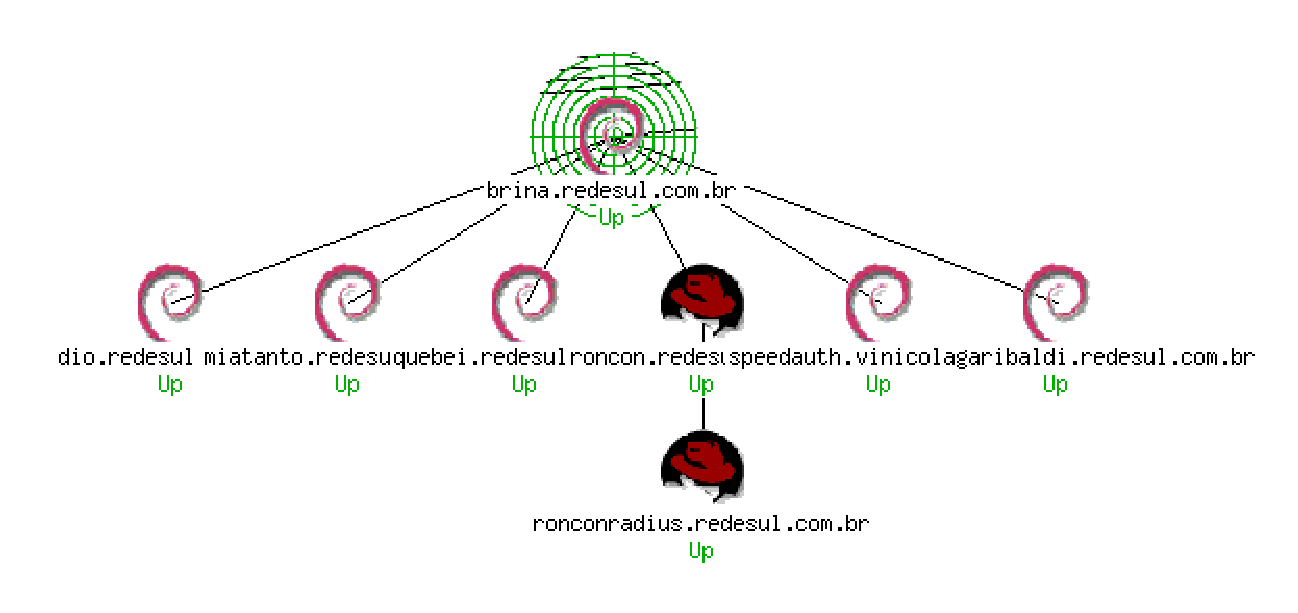
\includegraphics[width=380px]{img/servlog1.eps}
 \caption{Servidor de virtualização Brina. REFAZER ???}
 \label{fig:servlog1}
\end{figure}

O servidor chamado Fulmine executa doze \ac{VM}s (Figura \ref{fig:servlog2}), que fornecem os seguintes serviços:
\begin{itemize}
 \item \textit{Backup}: sua configuração é 1 \textit{core} para processamento, 2 GB de memória e X GB de disco. Nele é executado o serviço 
 de \textit{backup} dos equipamentos do provedor, para isso é utilizado \textit{scripts} que buscam e copiam os dados por \ac{FTP};
 \item \ac{DNS} autoritativo secundário: fornece o serviço de \ac{DNS} autoritativo dos domínios hospedados pela empresa;
 \item \ac{DNS} recursivo primário: fornece o serviço de \ac{DNS} para clientes de todo o provedor;
 \item Gerência \textit{Hotspot}: Servidor de gerência de equipamentos da Ubiquiti que fazem hotspot utilizado pelo provedor;
 \item Hospedagem sites \ac{WHM}: serviços de hospedagens de sites e banco de dados gerenciados pelo \ac{WHM};
 \item \ac{IPv6}: fornece o serviço de \ac{DNS} e \ac{NAT} para navegação \ac{IPv6} do provedor;
 \item Monitoramento \ac{PRTG}: serviço de monitoramento de tráfego e equipamentos da rede \textit{core} do provedor;
 \item \textit{Radius} \ac{ADSL}: Serviço de autenticação \ac{ADSL} de terceiros utilizando \textit{radius};
 \item \textit{Radius} autenticação \ac{PPPoE}: Serviço de autenticação \ac{PPPoE} do provedor utilizando \textit{radius};
 \item Telefonia: serviço de telefonia (central telefônica) \textit{Asterisk} do provedor;
 \item \textit{Terminal service}: \textit{terminal service} para suporte e gerência de fibra óptica do provedor;
\end{itemize}

\begin{figure}[h!]
 \centering
 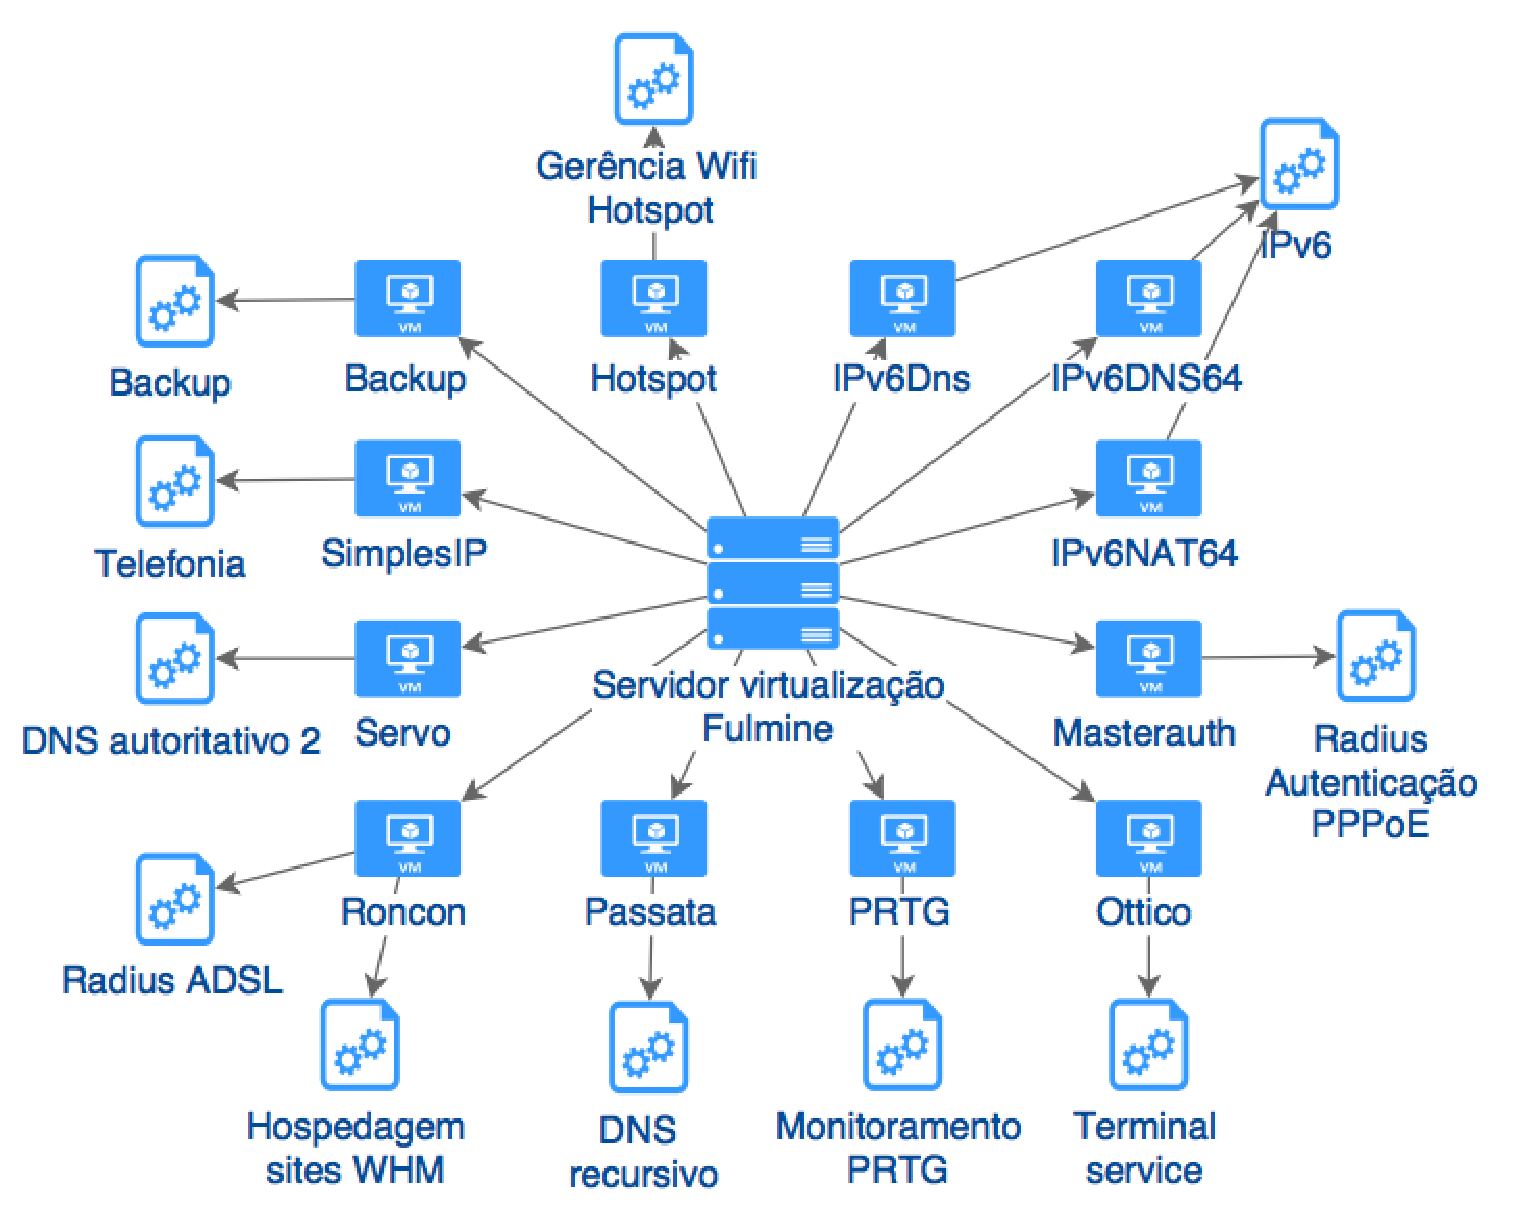
\includegraphics[width=430px]{img/servlog2.eps}
 \caption{Servidor de virtualização Fulmine.}
 \label{fig:servlog2}
\end{figure}

-graficos cpu memoria disco cada servidor de virtualizacao?? colocar aqui ou na implementacao?

-citar ferramentas monitoramento, update e backup??

\section{Serviços críticos}
\label{section:servcrit}

Na seção anterior foram detalhados todos os serviços que estão atualmente disponíveis na empresa, com isso nesta seção será feito a idenficação
dos serviços mais críticos para a empresa.

Para selecionar os serviços críticos anteriormente foi detalhado todos os serviços, sendo que os seguintes critérios foram utilizados: 
NAO COLOCAR EM ITENS ?? 
a quantidade de usuários ou funcionários que utilizam o serviço; 
o número de requisições em um determinado tempo;
o volume de objetos do serviço;
a quantidade de transações.
Deste modo, pode-se afirmar que esses critérios são importantes, pois caso os serviços relacionados a eles ficarem indisponíveis causarão 
um prejuízo financeiro para a empresa. 

Os serviços estão listados a seguir e ordenados por relevância:
\begin{itemize}
 \item \ac{DNS} primário: este serviço foi classificado como mais importante pois possui um impacto direto nos clientes do provedor, que 
 totalizam aproximadamente 9000 clientes. Sendo um provedor de internet, sua prioridade é fornecer uma navegação de qualidade aos seus clientes, 
 sabendo que o \ac{DNS} é fundamental para essa navegação, assim caracterizando essa importante classificação. Outro importante critério é
 o número de requisições por segundo (Figura ??), que é o maior entre todos os outros serviços.
 \item \textit{Radius}: 
 \item Sistemas: 
 \item telefonia: 
\end{itemize}

Tendo esses serviços pode-se identificar quais máquinas virtuais serão incluídas no ambiente de alta disponibilidade...


Esboço: \\
-DNS (impacto direto para clientes e rede interna): \\
requisicoes por segundo\\
numero de usuarios\\
-Radius (impacto direto para clientes): \\
numero de usuarios autentidados em x tempo\\
quantidade de dados armazenados no db em x tempo, trafego utilizado, tempo conexao\\
numero de usuarios\\
-Sistemas (impacto indireto para clientes): \\
gasto com funcionarios ociosos\\
quantidade de atendimento a clientes\\
numero de cobrancas enviadas para clientes efetuar pagamento\\
comunicacao entre setores e funcionarios\\
numero de usuarios\\
-Telefonia (impacto indireto para clientes): \\
quantidade de atendimento a clientes\\
comunicacao entre setores e funcionarios\\
ligacoes saintes, atendimento, cobranca, tecnicos instalacoes internet\\
numero de usuarios\\

Exibir disponibilidade média atual dos serviços, com gráficos



%A Tabela \ref{tab:servporservidor} mostra todos os servidores, incluindo virtuais, e seus respectivos serviços.
%\begin{table}
%\caption {Serviços por servidor}
%\label{tab:servporservidor}
%\begin{center}
%\begin{tabular}{|l|p{12cm}|}\hline
%Servidor & Descrição\\\hline
%asp & Servidor web linguagem ASP\\\hline
%backup & Servidor de backup equipamentos de rede do provedor\\\hline
%bello & Servidor de storage do bacula, para backup dos outros servidores\\\hline
%brina & Servidor de virtualização\\\hline
%cacti & Servidor de monitoramento da rede do provedor\\\hline
%cactibackbone & Servidor de monitoramento da rede do provedor\\\hline
%dati & Banco de dados dos servidores de e-mail e cameras\\\hline
%dio & Servidor de hospedagem de sites PHP4\\\hline
%esibire & Servidor de hospedagem de vídeos\\\hline
%fatefurbo & Servidor para gerência da fibra óptica do provedor\\\hline
%fiberhome & Servidor para gerência da fibra óptica do provedor\\\hline
%fulmine & Servidor de virtualização\\\hline
%hotspot & Servidor de gerência de equipamentos da Ubiquiti que fazem hotspot utilizado pelo provedor\\\hline
%ledriovardar & Servidor de terminal service do suporte e gerência do provedor\\\hline
%masterauth & Servidor de autenticação PPPoE do provedor\\\hline
%merak & Servidor de e-mail\\\hline
%miatanto & Servidor de streaming Icecast para web rádio\\\hline
%mondoperso & Servidor de streaming Icecast de uma rádio ao vivo\\\hline
%monete & Servidor de hospedagem de site dedicada do provedor\\\hline
%monit & Servidor de monitoramento e gráficos de todos servidores\\\hline
%nino & Ambiente de desenvolvimento para setor de programação web\\\hline
%ns & Servidor primário de DNS autoritativo\\\hline
%ottico & Servidor de terminal service do suporte e gerência de fibra óptica do provedor\\\hline
%parla & Servidor de mensagens instantâneas XMPP do provedor\\\hline
%passata & Servidor primário de DNS recursivo do provedor\\\hline
%passata2 & Servidor secundário de DNS recursivo do provedor\\\hline
%piova & Servidor de virtualização\\\hline
%pomodoro & Servidor de documentação Sakai do provedor\\\hline
%postfix & Servidor de SMTP para envio de e-mail marketing\\\hline
%quebei & Servidor de gerência do bacula, para backup dos outros servidores\\\hline
%raggio & Servidor de virtualização\\\hline
%rauco & Servidor de hospedagens WHM\\\hline
%roncon & Servidor de hospedagens WHM\\\hline
%ronconradius & Servidor de radius ADSL de terceiros\\\hline
%servo & Servidor secundário de DNS autoritativo\\\hline
%servo6 & Servidor terciário de DNS autoritativo\\\hline
%sfrunhon & Servidor de gráficos para monitoramento de clientes do provedor\\\hline
%simplesip & Servidor de telefonia Asterisk do provedor\\\hline
%soldi & Servidor de sistemas do provedor e outros ERPs\\\hline
%speedauth & Servidor de autenticação PPPoE do provedor\\\hline
%tempesta & Servidor de virtualização\\\hline
%trapel & Servidor de teste de banda do provedor\\\hline
%tuono & Servidor de virtualização\\\hline
%venti & Servidor de virtualização\\\hline
%vigilante & Servidor de reprodução e armazenamento das câmeras do provedor\\\hline
%vinicolag & Servidor de backup de um cliente\\\hline
%\end{tabular}
%\end{center}
%\end{table}
